% !TeX root = main.tex

% main.tex
% header.tex
\documentclass[a4paper,11pt,twoside,ngerman,xcolor]{book}
\usepackage[a4paper,left=3.5cm,right=2.5cm,bottom=3.5cm,top=3cm]{geometry}

\usepackage[german,english]{babel}

\usepackage[pdftex]{graphicx,xcolor}
\usepackage{amsmath,amssymb,subfigure}

\usepackage{pdfpages}
\usepackage[hidelinks]{hyperref}


% Theorem-Umgebungen
\usepackage[amsmath,thmmarks]{ntheorem}

% Korrekte Darstellung der Umlaute
\usepackage[utf8]{inputenc}
\usepackage[T1]{fontenc}

% Algorithmen
\usepackage[chapter]{algorithm}
\usepackage{algorithmic}

\usepackage{enumerate}


% Bibtex deutsch
\usepackage{bibgerm}
\usepackage[numbers]{natbib}

% URLs
\usepackage{url}

% Caption Packet
\usepackage[margin=0pt,font=small,labelfont=bf]{caption}
% Gliederung einstellen
%\setcounter{secnumdepth}{5}
%\setcounter{tocdepth}{5}

% Theorem-Optionen %
\theoremseparator{.}
\theoremstyle{change}
\newtheorem{theorem}{Theorem}[section]
\newtheorem{satz}[theorem]{Satz}
\newtheorem{lemma}[theorem]{Lemma}
\newtheorem{korollar}[theorem]{Korollar}
\newtheorem{proposition}[theorem]{Proposition}
% Ohne Numerierung
\theoremstyle{nonumberplain}
\renewtheorem{theorem*}{Theorem}
\renewtheorem{satz*}{Satz}
\renewtheorem{lemma*}{Lemma}
\renewtheorem{korollar*}{Korollar}
\renewtheorem{proposition*}{Proposition}
% Definitionen mit \upshape
\theorembodyfont{\upshape}
\theoremstyle{change}
\newtheorem{definition}[theorem]{Definition}
\theoremstyle{nonumberplain}
\renewtheorem{definition*}{Definition}
% Kursive Schrift
\theoremheaderfont{\itshape}
\newtheorem{notation}{Notation}
\newtheorem{konvention}{Konvention}
\newtheorem{bezeichnung}{Bezeichnung}
\theoremsymbol{\ensuremath{\Box}}
\newtheorem{beweis}{Beweis}
\theoremsymbol{}
\theoremstyle{change}
\theoremheaderfont{\bfseries}
\newtheorem{bemerkung}[theorem]{Bemerkung}
\newtheorem{beobachtung}[theorem]{Beobachtung}
\newtheorem{beispiel}[theorem]{Beispiel}
\newtheorem{problem}{Problem}
\theoremstyle{nonumberplain}
\renewtheorem{bemerkung*}{Bemerkung}
\renewtheorem{beispiel*}{Beispiel}
\renewtheorem{problem*}{Problem}

% Algorithmen anpassen %
\renewcommand{\algorithmicrequire}{\textit{Eingabe:}}
\renewcommand{\algorithmicensure}{\textit{Ausgabe:}}
\floatname{algorithm}{Algorithmus}
\renewcommand{\listalgorithmname}{Algorithmenverzeichnis}
\renewcommand{\algorithmiccomment}[1]{\textcolor{gray}{// #1}}

% Zeilenabstand einstellen %
\renewcommand{\baselinestretch}{1.25}
% Floating-Umgebungen anpassen %
\renewcommand{\topfraction}{0.9}
\renewcommand{\bottomfraction}{0.8}
% Abkuerzungen richtig formatieren %
\usepackage{xspace}
\newcommand{\vgl}{vgl.\@\xspace} 
\newcommand{\zB}{z.\nolinebreak[4]\hspace{0.125em}\nolinebreak[4]B.\@\xspace}
\newcommand{\bzw}{bzw.\@\xspace}
\newcommand{\dahe}{d.\nolinebreak[4]\hspace{0.125em}h.\nolinebreak[4]\@\xspace}
\newcommand{\etc}{etc.\@\xspace}
\newcommand{\evtl}{evtl.\@\xspace}
\newcommand{\ggf}{ggf.\@\xspace}
\newcommand{\bzgl}{bzgl.\@\xspace}
\newcommand{\so}{s.\nolinebreak[4]\hspace{0.125em}\nolinebreak[4]o.\@\xspace}
\newcommand{\iA}{i.\nolinebreak[4]\hspace{0.125em}\nolinebreak[4]A.\@\xspace}
\newcommand{\sa}{s.\nolinebreak[4]\hspace{0.125em}\nolinebreak[4]a.\@\xspace}
\newcommand{\su}{s.\nolinebreak[4]\hspace{0.125em}\nolinebreak[4]u.\@\xspace}
\newcommand{\ua}{u.\nolinebreak[4]\hspace{0.125em}\nolinebreak[4]a.\@\xspace}
\newcommand{\og}{o.\nolinebreak[4]\hspace{0.125em}\nolinebreak[4]g.\@\xspace}
\newcommand{\oBdA}{o.\nolinebreak[4]\hspace{0.125em}\nolinebreak[4]B.\nolinebreak[4]\hspace{0.125em}d.\nolinebreak[4]\hspace{0.125em}A.\@\xspace}
\newcommand{\OBdA}{O.\nolinebreak[4]\hspace{0.125em}\nolinebreak[4]B.\nolinebreak[4]\hspace{0.125em}d.\nolinebreak[4]\hspace{0.125em}A.\@\xspace}

% Leere Seite ohne Seitennummer, naechste Seite rechts
\newcommand{\blankpage}{
 \clearpage{\pagestyle{empty}\cleardoublepage}
}

% Keine einzelnen Zeilen beim Anfang eines Abschnitts (Schusterjungen)
\clubpenalty = 10000
% Keine einzelnen Zeilen am Ende eines Abschnitts (Hurenkinder)
\widowpenalty = 10000 \displaywidowpenalty = 10000
% EOF

\begin{document}
\selectlanguage{german}
\begin{titlepage}
\definecolor{TUGreen}{rgb}{0.517,0.721,0.094}
\vspace*{-2cm}
\newlength{\links}
\setlength{\links}{-1.5cm}
\sffamily
\hspace*{\links}
\begin{minipage}{12.5cm}

\includegraphics[width=8cm]{bilder/tud_logo_rgb}
%\hspace*{-0.25cm} \textbf{TECHNISCHE UNIVERSIT"AT DORTMUND}\\
%\hspace*{-1.2cm} \rule{5mm}{5mm} \hspace*{0.1cm} FACHBEREICH INFORMATIK\\
\end{minipage}

\vspace*{4cm}

\hspace*{\links}
\hspace*{-0.2cm}
\begin{minipage}{9cm}
\large
\begin{center}
{\Large Bachelorarbeit} \\
\vspace*{1cm}
\textbf{Parallelisierung einer speichereffizienten Approximation der LZ77-Faktorisierung} \\
\vspace*{1cm}
Gajann Sivarajah\\
% \vspace*{1cm}
\end{center}
\end{minipage}
\normalsize
\vspace*{5.5cm}

% \hspace*{\links}

\vspace*{2.1cm}

\hspace*{\links}
\begin{minipage}[b]{5cm}
% \normalsize
\raggedright
Gutachter: \\
Prof. Dr. Johannes Fischer \\
M.Sc. Patrick Dinklage \\
\end{minipage}

\vspace*{2.5cm}
\hspace*{\links}
\begin{minipage}[b]{8cm}
% \normalsize
\raggedright
Technische Universit"at Dortmund \\
Fakult"at f"ur Informatik\\
LS-11\\
http://afe.cs.tu-dortmund.de
\end{minipage}

\end{titlepage}

\blankpage
\pagenumbering{roman}
\tableofcontents
\cleardoublepage
\pagenumbering{arabic}
% Kapitel
% einleitung.tex
\chapter{Einleitung}
\section{Motivation und Hintergrund}
Die Entwicklung, Verbreitung und Nutzung digitaler Technologien hängt im hohen Maße von der Fähigkeit ab, große Mengen an Daten speichern, transportieren und
analysieren zu können. Der Umgang mit großen Datenmengen geht jedoch mit entsprechend hohen Kosten einher. Ein wichtiges Werkzeug zur Bewältigung dieses Problems
sind Kompressionstechniken, die Relationen und Redundanzen in Datenmengen extrahieren, um ihre Größe möglichst auf ihre inhärente Komplexität zu reduzieren. 
Im Laufe der Zeit wurden zahlreiche Kompressionsalgorithmen entwickelt, die wiederum über mehrere Iterationen verbessert wurden.Viele solcher Kompressionstechniken
können der Familie der LZ77-Algorithmen \cite{LemZiv} zugeordnet werden, wobei diese sich in Statistiken, wie der Laufzeit, der Speicheranforderung oder Kompressionrate unterscheiden
. In \cite{ApproxLZ77} wird eine Variante der LZ77-Faktorisierung beschrieben, die über drei Phasen eine 2-Approximation einer exakten LZ77-Faktorisierung
 \cite{exactLemZiv} erreichen kann. Diese beschränkten Einbußen in der Qualität der Ausgabe werden jedoch dadurch kompensiert, dass der Algorithmus die Speicheranforderung
weit unterbieten kann. In dieser Arbeit untersuchen wir diesen Algorithmus auf ihr Potential zur Parallelisierung.

\section{Ziele und Methodik}
Im Rahmen der Parallelisierung des approximativen LZ77-Algorithmus werden wir die erste Phase des Algorithmus dahingehend anpassen, dass mehrere Threads im 
shared-memory-Modell konfliktfrei auf Datenstrukturen zugreifen und eine korrekte Ausgabe liefern können. Im Rahmen der praktischen Evaluation der
beschriebenen Konzepte wird eine Implementierung in C++ herangezogen. Die Parallelisierung wird hauptsächlich über OpenMP-Instruktionen \cite{openmp} realisiert.
Im Rahmen dieser Arbeit wird insbesondere die parallele Generierung einer Suchtabelle von Referenzen, sowie die parallele Suche nach Referenzen über die gesamte Eingabe
hinweg betrachtet. Wir führen eine theoretische und praktische Evaluation der Qualität und Performanz der Algorithmen durch. Insbesondere stellen wir einen Vergleich der
Laufzeit und Speicheranforderung der sequentiellen und parallelen Approximation mit einer exakten LZ77-Faktorisierung \cite{exactLemZiv} an. Die Güte der Parallelisierung
werden wir anhand der gemessenen Beschleunigung der Laufzeit bewerten. Für jegliche Messungen verwenden wir Testdaten aus unterschiedlichen Kontexten des 
Pizza\& Chili Corpus \cite{corpus}.
\chapter{Grundlagen}

Zunächst stellen wir die verwendete Terminologie und relevante Konzepte bzw. Phänomene dar.

\section{Kompression} \label{comp}

\subsection{Verlustfreie Kompression}
Der Prozess der Kompression überführt eine Repräsentation einer finiten Datenmenge in eine möglichst kompaktere Form. Eine verlustfreie Kompression ist gegeben, falls die Abbildung
zwischen der ursprünglichen und komprimierten Datenmenge bijektiv ist. Die Korrektheit einer verlustfreien Kompression kann daher durch die Angabe einer Dekompressionsfunktion 
nachgewiesen werden. Ist diese Vorraussetzung nicht gegeben, so handelt es sich um eine verlustbehaftete Kompression, da eine Rekonstruktion der ursprünglichen Datenmenge nicht 
garantiert werden kann.

\subsection{Eingabe}
Unsere Eingabe sei durch eine $n$-elementige Zeichenfolge $S=e_1...e_n$ über dem numerischen Alphabet $\Sigma$ mit $e_i\in \Sigma$ $\forall i=1,...,n$ gegeben. Für jede
beliebige Zeichenfolge $S$ wird mit $|S|$ dessen Länge $n$ bezeichnet. Der Ausdruck $S[i..j]\in \Sigma^{j-i+1}$ mit $1\leq i\leq j\leq n$ beschreibt die Teilfolge $e_i...e_j$ ,
wobei im Falle, dass $i=j$ ist, das einzelne Zeichen $e_i$ referenziert wird. Alternativ kann ein einzelnes Zeichen $e_i$ auch durch $S[i]$ referenziert werden. Eine Teilfolge 
der Form $S[1..k]$ mit $k\leq n$ wird als Präfix von $S$ bezeichnet.

\subsection{Faktorisierung}
Ein charakteristisches Merkmal für die Klasse von Lempel-Ziv-Kompressionsverfahren ist die Repräsentation der Ausgabe in Form einer Faktorisierung. Für eine Eingabe $S=e_1...e_n$ 
wird eine Faktorisierung $S=f_1...f_z$ mit $z\leq n$ derart erzeugt, dass die Faktoren $S$ in eine equivalente Folge von nichtleeren Teilfolgen zerlegt werden. Hier ist jeder Faktor
$f_i$ mit $1\leq i\leq z$ als Präfix von $S[|f_1...f_i-1|+1..n]$ definiert, der bereits in $S[1..|f_1...f_i|]$ vorkommt oder als einzelnes Zeichen ohne vorheriges Vorkommen. Die im 
Folgenden betrachteten Algorithmen können speziell der Klasse der LZ77-Kompressionsverfahren zugeordnet werden, dessen Faktoren im Schema des Lempel-Ziv-Storer-Szymanski repräsentiert
werden sollen. Zur Darstellung von Referenzen wird das Tupel $(len, pos)$ verwendet, wobei $pos$ die Position des vorherigen Vorkommens und $len>0$ die Länge des Faktors beschreibt. 
Einzelne Zeichen können wiederum durch das Tupel $(0, e)$ mit $e\in \Sigma$ dargestellt werden.

\subsection{Binäre (De-)Kodierung}
Die Abbildung $Bin_{IO}: \Sigma^* \rightarrow N$ gibt die Anzahl der Bits für die Kodierung einer beliebigen Zeichenfolge an. Im Rahmen dieser Arbeit gehen wir davon aus, dass die 
Eingabe $S$ in binärer Form vorliegt und auf dem Alphabet $\Sigma=\{1,...,255\}$ erzeugt wurde. Jedes Zeichen wird durch 8 Bits, oder 1 Byte, dargestellt und erlaubt einen 
Offline-Zugriff. Die gesamte binäre Eingabegröße sei damit gegeben durch 

\begin{equation}
    N_{Bin} = \sum_{i=1}^{|S|} Bin_{IO}(S[i]) = 8*|S|.
\end{equation}
Die eingelesene Eingabefolge wird durch den Kompressionsalgorithmus in die Faktorfolge $S=f_1...f_z$ überführt. Jeder Faktor $f_i$, der Form $(len, pos)$ oder $(0, e)$, werde 
durch $Bin_{IO}(f_i)$ Bits kodiert. Die binäre Ausgabegröße ergibt sich aus dem Ausdruck
\begin{equation}
    Z_{Bin} = \sum_{i=1}^{z} Bin_{IO}(f_i).
\end{equation}
, wobei die Anzahl der Bits für die Kodierung der Faktoren $f_i$ durch den Kompressionsalgorithmus und der Kodierungsstrategie bestimmt wird.

\subsection{Metriken}
Die Qualität einer Kompression kann durch verschiedene Metriken quantifiziert werden. Zum Einen beschreibt die Kompressionsrate $CR$ den Grad der Kompression und ist durch den
Ausdruck, 
\begin{equation}
    CR = \frac{Z_{Bin}}{N_{Bin}}
\end{equation}
, definiert.
Da die Kodierung der Faktoren nicht eindeutig aus der Wahl des Kompressionsalgorithmus eingegrenzt wird, ist stattdessen die Anzahl der erzeugten Faktoren ein
weiteres geeignetes Gütemaß. Für die Eingabe $S$ der Länge n und der Ausgabe $f_1...f_z$ sei die Faktorrate durch
\begin{equation}
    FR = \frac{z}{n}
\end{equation}
gegeben. In beiden Fällen wird ein niedriger Wert bevorzugt, da dieser auf eine bessere Extraktion von Redundanzen hinweist.

\section{Parallelität}
Das Ziel dieser Arbeit ist die Entwicklung und Evaluation eines parallel Kompressionsalgorithmus. Im Folgenden definieren wir die Rahmenbedingungen und Konzepte der Parallelität.

\subsection{Shared-Memory-Modell}
Unser Algorithmus agiere auf einem Shared-Memory-Modell mit $P$ Ausführungseinheiten, welches im Gegensatz zum Distributed-Memory-Modell allen beteiligten Ausführungseinheiten bzw. 
Prozessoren einen gemeinsamen Zugriff auf den Speicher ermöglicht. Im Rahmen der Arbeit und Kommunikation unter den Prozessoren wird man jedoch auf Konflikte bei gleichzeitigen 
Speicherzugriffen zustoßen. Ein parallel modellierter Algorithmus muss explizit hinsichtlich der Korrektheit und Effizienz Mechanismen zur Synchronisation implementieren.

\subsection{Metriken}
Das Ziel der Parallelisierung eines Algorithmus liegt hauptsächlich in einer Verbesserung der Laufzeit, insbesondere unter Berücksichtigung von Ressourcenkonflikten. Die zeitliche
Beschleunigung der Laufzeit kann durch den Speedup $SP$ bemessen werden. Für eine Eingabe $S$ der Länge n brauche ein sequenzieller Durchlauf $T(n, p=1)$ Zeit, während ein paralleler
Algorithmus mit $P$ Prozessoren $T(n,p=P)$ an Zeit benötigt. Der Speedup ist dabei definiert durch
\begin{equation}
    SP(n,P) = \frac{T(n,1)}{T(n,P)}.
\end{equation}


\chapter{Kompressionsalgorithmen}

\section{(exakte) LZ77-Kompression}
Die resultierende Faktorisierung aus der exakten LZ77-Kompression wird im Folgenden als Referenz für die Evaluation der Ergebnisse anderer Algorithmen verwendet.
Zusätzlich zu der bereits beschriebenen Struktur von Faktorisierung nach dem Lempel-Ziv-Schema erfüllen referierende Faktoren die Eigenschaft, dass sie stets
die längste Zeichenfolge referenzieren, die ein vorheriges Vorkommen hat. Der Algorithmus hat hat damit einen Greedy-Charakter. Im Rahmen der Evaluation nutzen 
wir Implementierung des Algorithmus, welcher auf der Erzeugung eines Suffixarray basiert. Für eine Eingabe der Länge $n$ kann die Laufzeit des Algorithmus auf
$O(n)$ geschätzt werden. Der eingespannter Speicher kann auch auf $O(n)$ geschätzt werden, wobei in der Praxis ein großer konstanter Faktor zu erwarten ist.
\chapter{Praktische Evaluation}

\section{Experimentelle Umgebung}
Die folgenden Experimente wurden auf Ubuntu 24.04 auf einem Rechner mit 16 ???? Prozessoren und 128GB RAM durchgeführt. Die C++-Implementierung wurde
mithilfe von GCC in der Version 13.1 kompiliert.

\section{Implementierung}
Die Implementierung der Algorithmen erfolgte im C++20-Standard.

\section{Daten}
Die Experimente wurden auf verschiedenen Datenbausteinen vom Pizza \& Chili-Corpus durchgeführt. Die verwendeten Datenbausteine sind in der folgenden Tabelle aufgelistet.

\begin{center}
    \begin{tabular}{|c|c|c|c|c|}
        \hline
        \textbf{Datei} & \textbf{Größe} & \textbf{Alphabet} & \textbf{Beschreibung} \\
        \hline
        \hline
        \texttt{dna} & 100MB & 4 & DNA-Sequenzen \\
        \hline
        \texttt{english} & 100MB & 256 & Englische Texte \\
        \hline
        \texttt{proteins} & 100MB & 20 & Proteinsequenzen \\
        \hline
        \texttt{sources} & 100MB & 256 & Quellcode \\
        \hline
        \texttt{xml} & 100MB & 256 & XML-Dateien \\
        \hline
    \end{tabular}
\end{center}
Es handelt sich hierbei um Präfixe der Originaldateien, die im Pizza \& Chili-Corpus enthalten sind.

\section{Ergebnisse}
Die Ergebnisse der Experimente sind in den folgenden Tabellen und Abbildungen dargestellt.\\
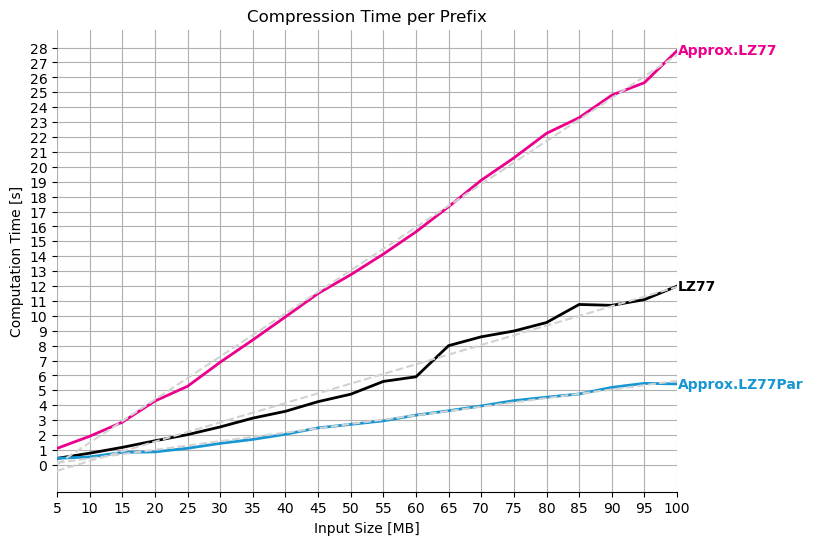
\includegraphics[scale = 0.65]{bilder/progressive.png}\\
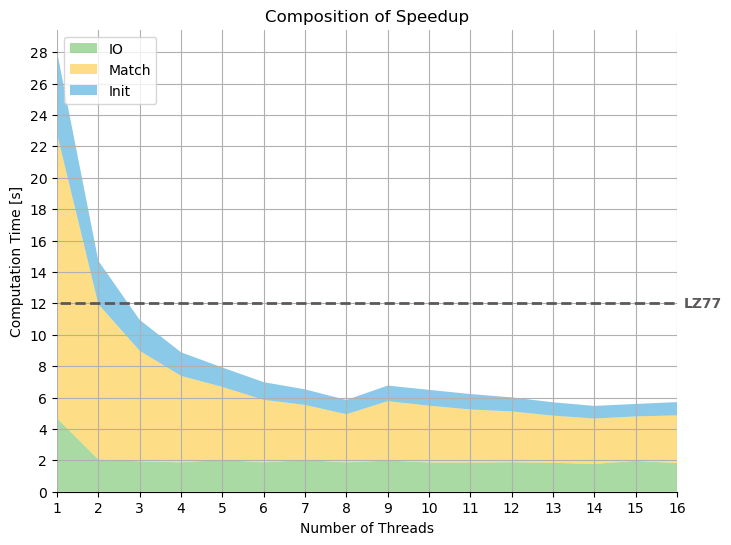
\includegraphics[scale = 0.65]{bilder/progressive_speedup_stack.png}\\
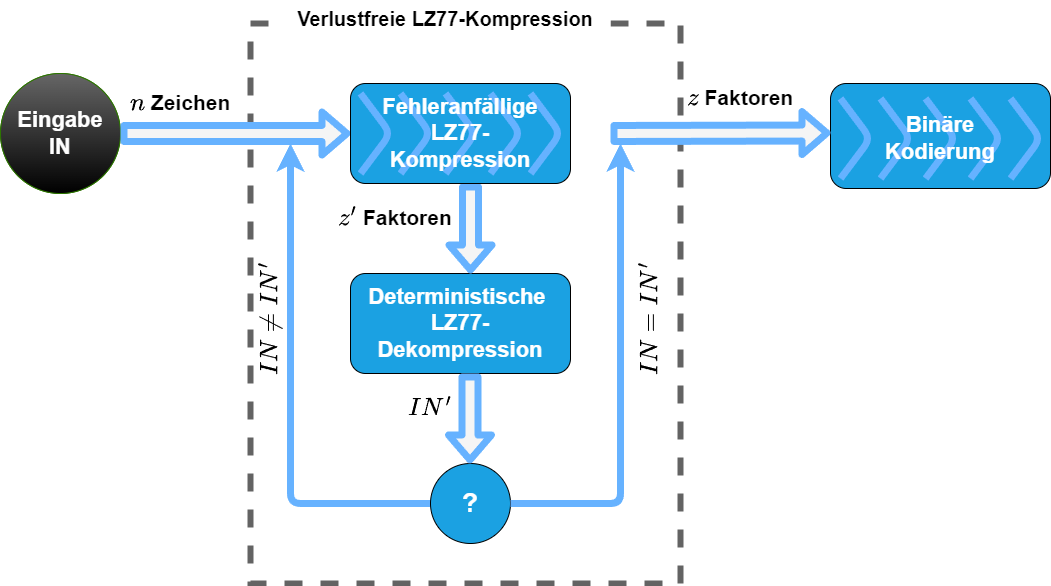
\includegraphics[scale = 0.4]{bilder/lasvegas_algorithm.png}
% Anhang
\appendix
% anhang.tex
\chapter{Weitere Informationen}
\section{Alternative Eingabedaten} \label{alternative}
Im Folgenden sind die vollständigen Laufzeitmessungen für die Eingabedaten, sources, english, dna und xml, aufgeführt. Während die absoluten Werte
der Laufzeit für die verschiedenen Eingabedaten variieren, zeigen die Kurven der Laufzeitmessungen eine ähnliche Tendenz.
\begin{figure} [H]
    \centering
    \caption{Laufzeitmessung von LZ77, Approx.LZ77 und Approx.LZ77Par(16 Threads) auf verschiedenen Präfixen von sources. Als Vergleichsmaß wurde 
    die lineare Regression der Kurven gestrichelt eingezeichnet.}
    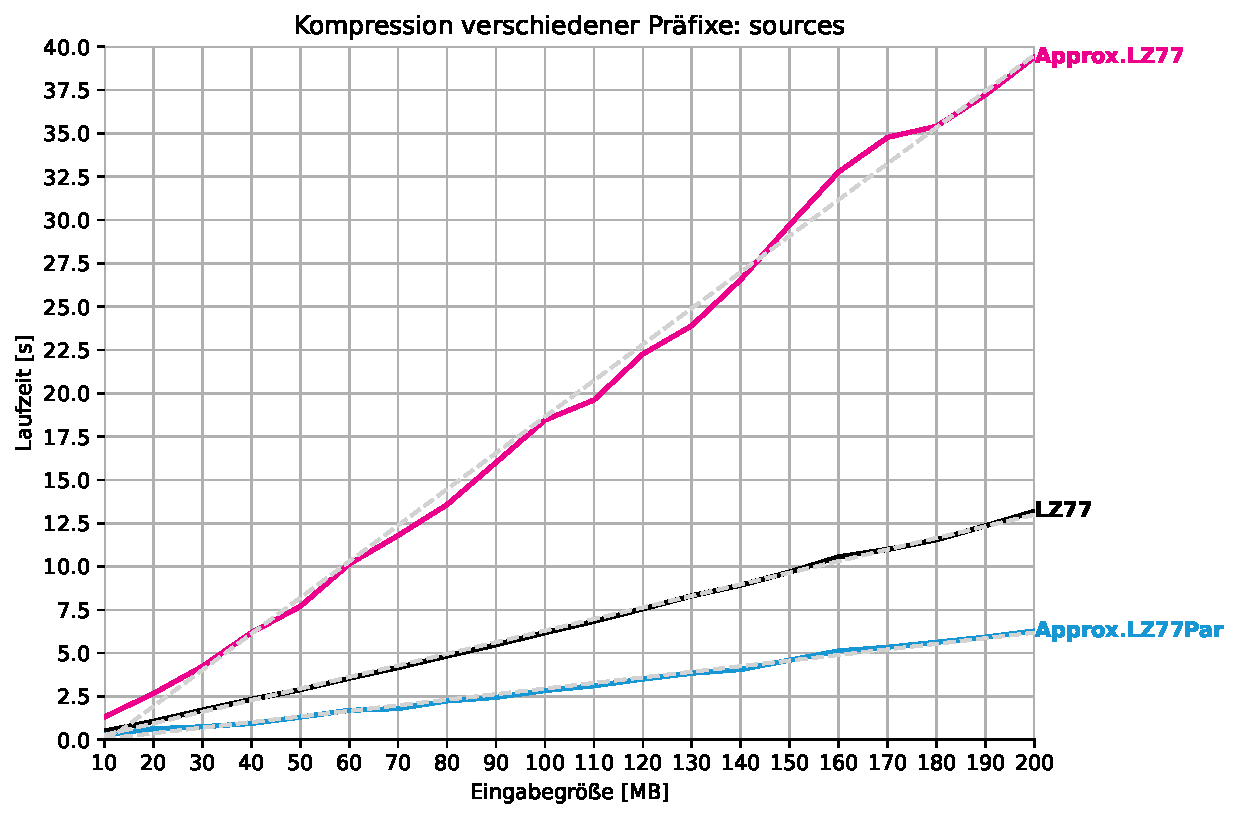
\includegraphics[scale=0.65]{Images/progressive_sources.pdf}
\end{figure}

\begin{figure}[H]
    \centering
    \caption{Laufzeitmessung von Approx.LZ77Par mit verschiedener Anzahl an Threads für sources}
    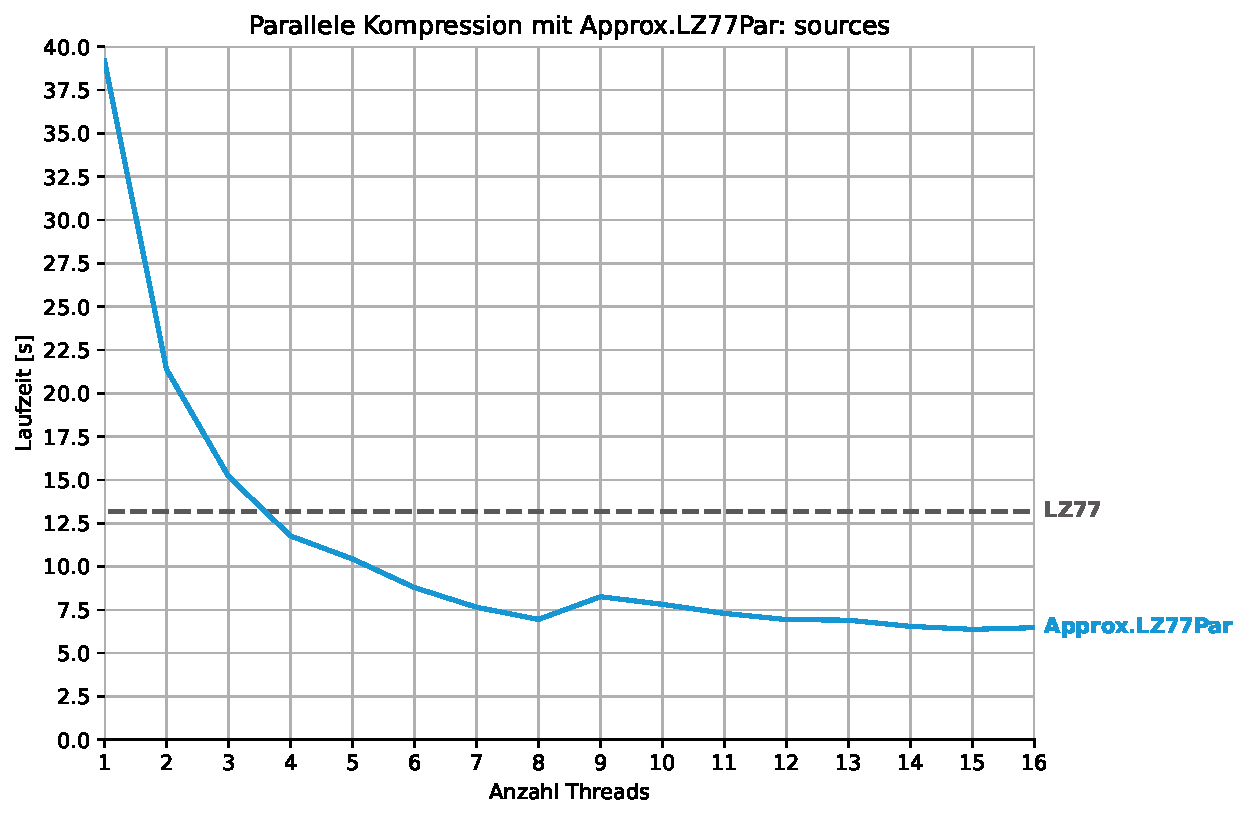
\includegraphics[scale=0.65]{Images/progressive_speedup_sources.pdf}
\end{figure}

\begin{figure}[H]
    \centering
    \caption{Laufzeitmessung von LZ77, Approx.LZ77 und Approx.LZ77Par(16 Threads) auf verschiedenen Präfixen von english. Als Vergleichsmaß wurde 
    die lineare Regression der Kurven gestrichelt eingezeichnet.}
    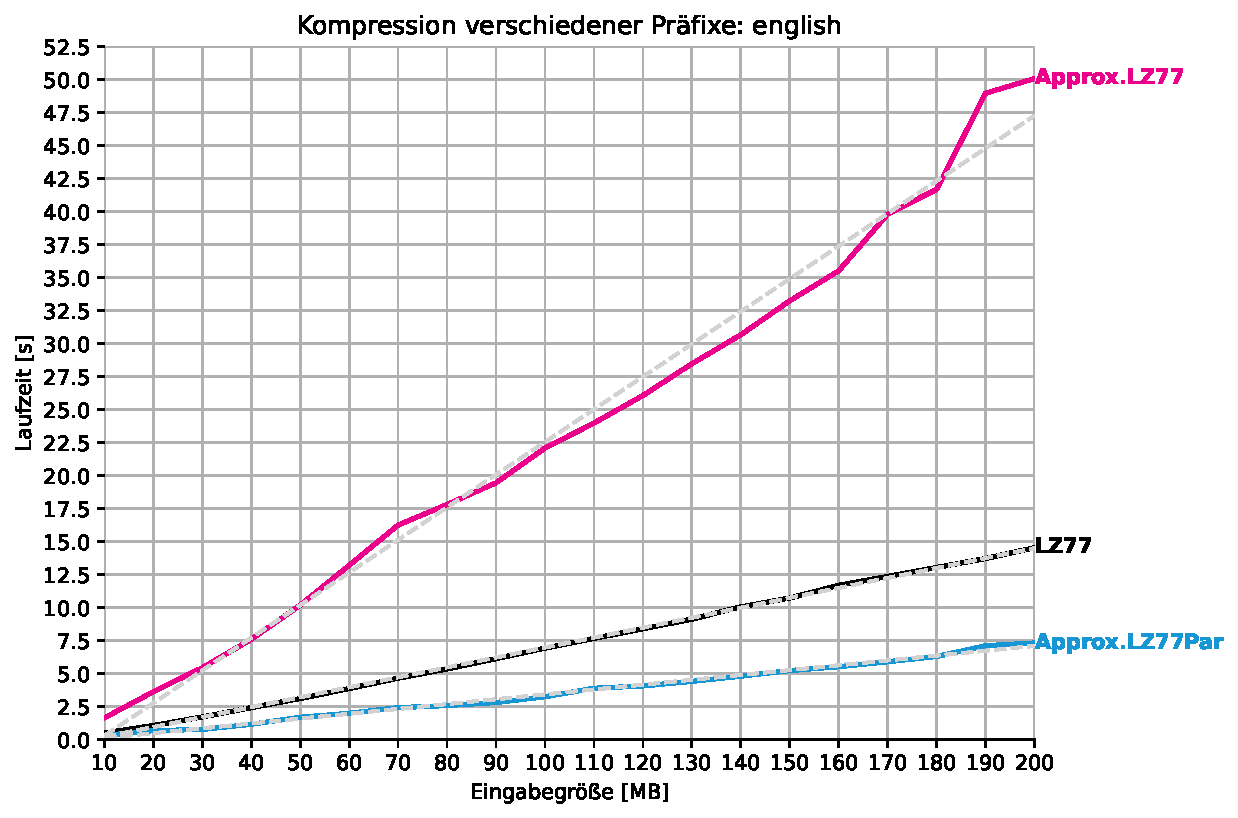
\includegraphics[scale=0.65]{Images/progressive_english.pdf}
\end{figure}

\begin{figure}[H]
    \centering
    \caption{Laufzeitmessung von Approx.LZ77Par mit verschiedener Anzahl an Threads für english}
    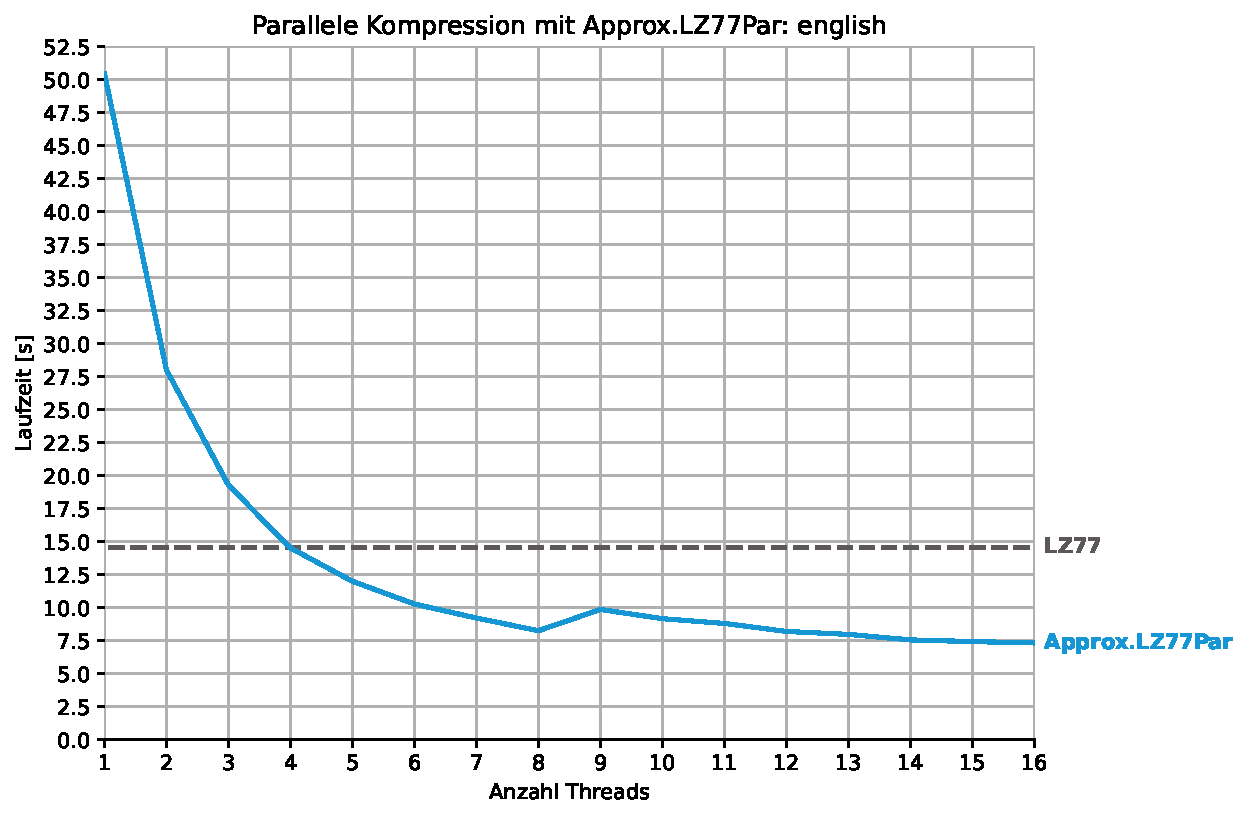
\includegraphics[scale=0.65]{Images/progressive_speedup_english.pdf}
\end{figure}

\begin{figure}[H]
    \centering
    \caption{Laufzeitmessung von LZ77, Approx.LZ77 und Approx.LZ77Par(16 Threads) auf verschiedenen Präfixen von dna. Als Vergleichsmaß wurde 
    die lineare Regression der Kurven gestrichelt eingezeichnet.}
    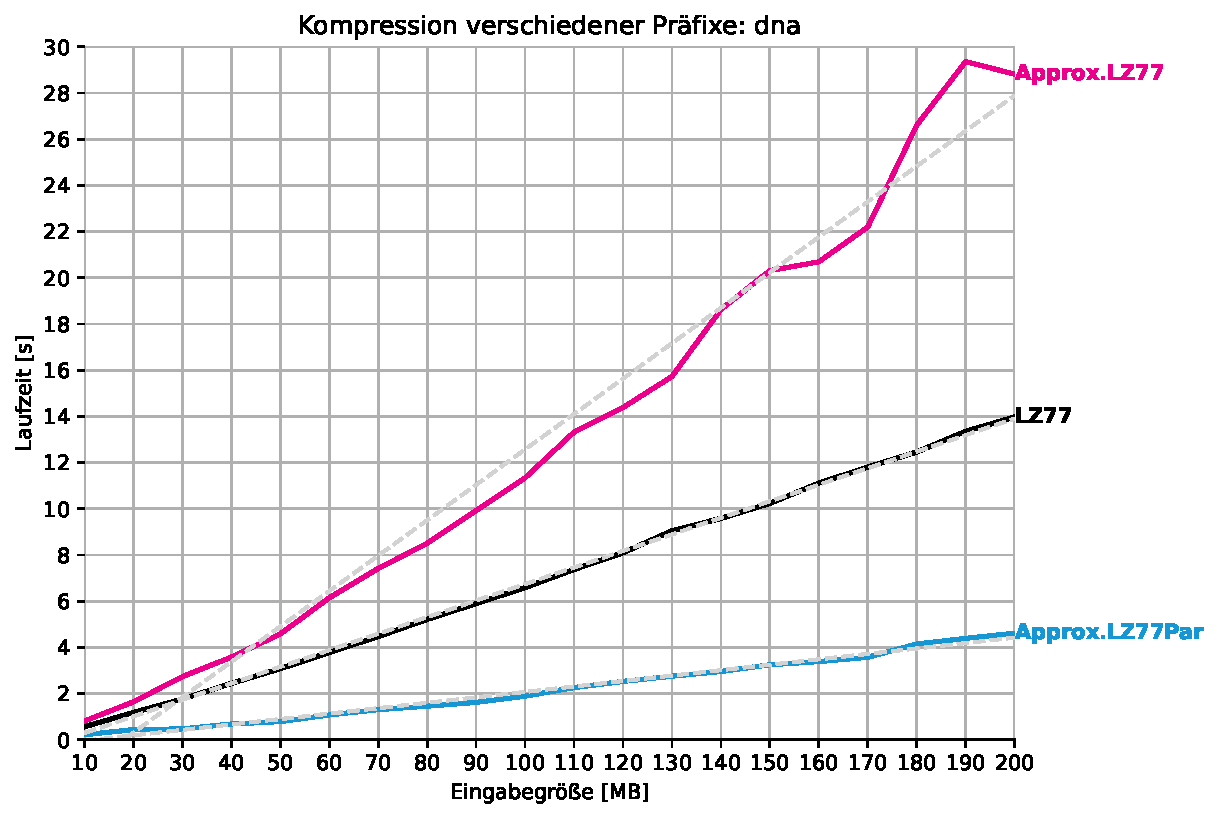
\includegraphics[scale=0.65]{Images/progressive_dna.pdf}
\end{figure}

\begin{figure}[H]
    \centering
    \caption{Laufzeitmessung von Approx.LZ77Par mit verschiedener Anzahl an Threads für dna}
    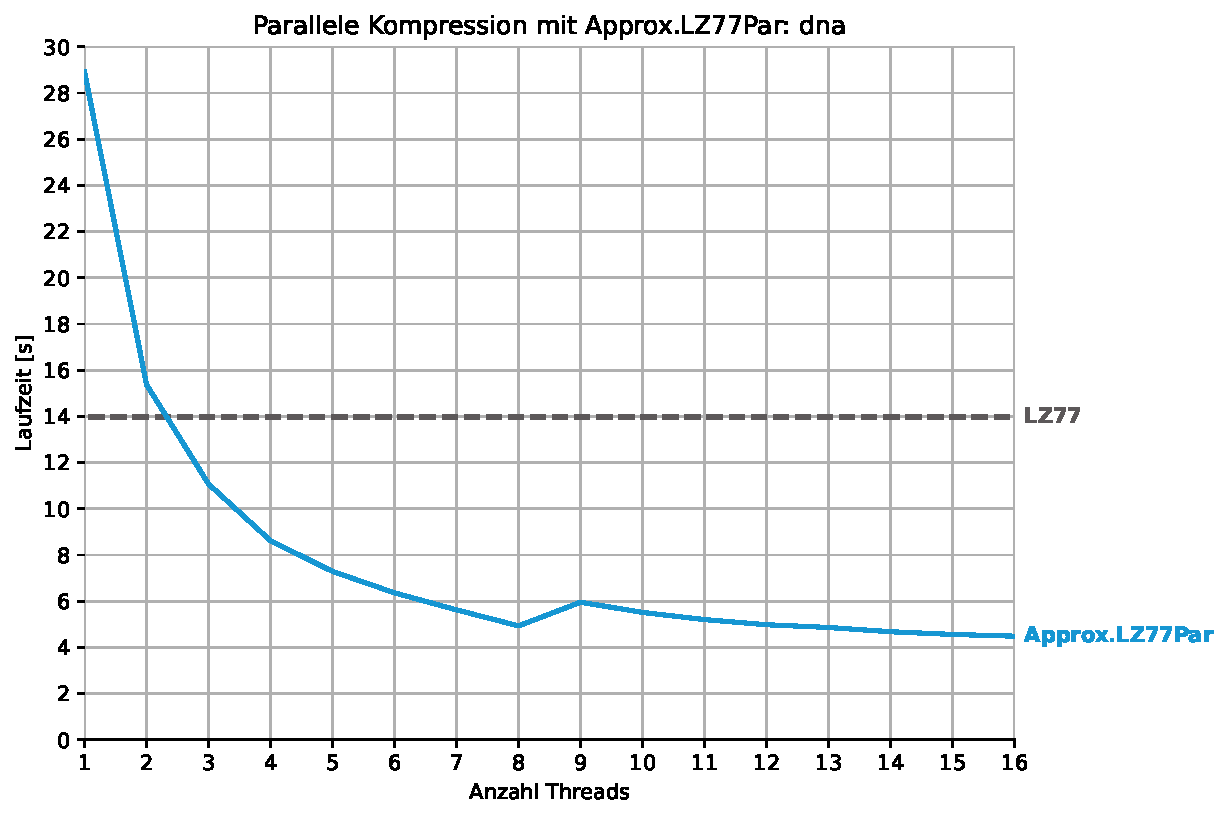
\includegraphics[scale=0.65]{Images/progressive_speedup_dna.pdf}
\end{figure}

\begin{figure}[H]
    \centering
    \caption{Laufzeitmessung von LZ77, Approx.LZ77 und Approx.LZ77Par(16 Threads) auf verschiedenen Präfixen von xml. Als Vergleichsmaß wurde 
    die lineare Regression der Kurven gestrichelt eingezeichnet.}
    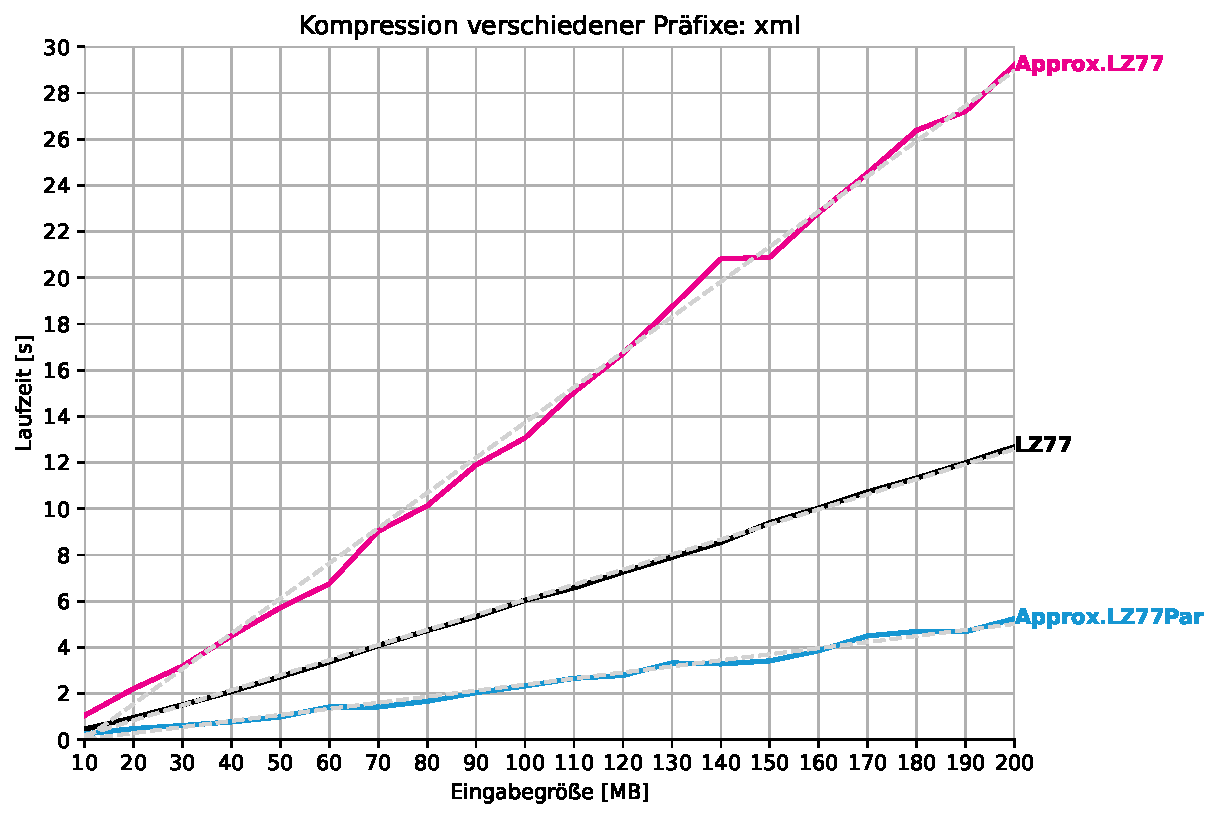
\includegraphics[scale=0.65]{Images/progressive_xml.pdf}
\end{figure}

\begin{figure}[H]
    \centering
    \caption{Laufzeitmessung von Approx.LZ77Par mit verschiedener Anzahl an Threads für xml}
    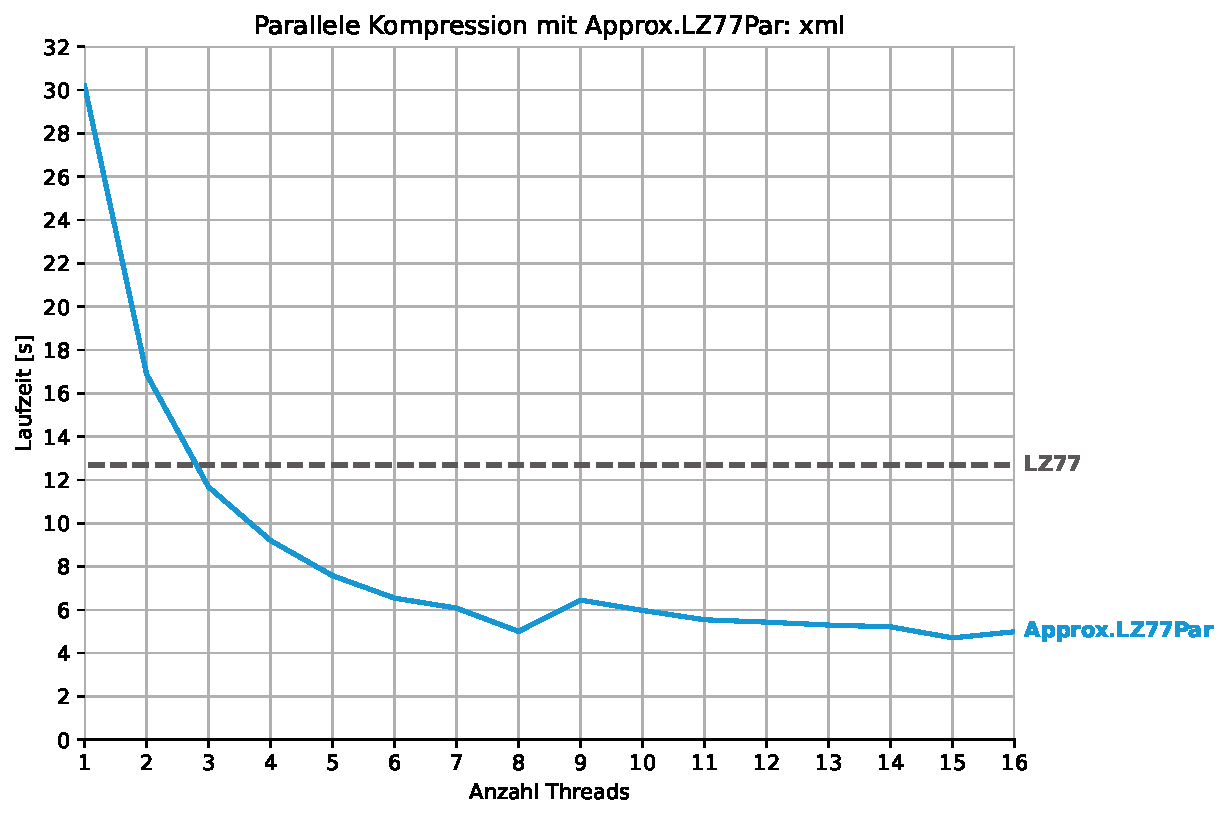
\includegraphics[scale=0.65]{Images/progressive_speedup_xml.pdf}
\end{figure}
\pagebreak
\section{Alternative Testumgebung}
Für die folgenden Messwerte wurden die Algorithmen auf einem Rechner mit einem AMD EYPC 7452 32-Core Prozessor mit 128 nutzbaren Threads ausgeführt.
Die Einstellungen der Algorithmen, die in \ref{settings} etabliert wurden, wurden beibehalten.

\begin{table}[ht]
    \centering
    \caption{Messwerte der Algorithmen auf verschiedenen Eingabedateien}
    \begin{tabular} { |c|c|c|c|c|c| }
        \hline
        \textbf{Eingabe} & \textbf{Algorithmus} & \textbf{Laufzeit[s]} & \textbf{Speicher} & \textbf{FR} & \textbf{CR*} \\
        \hline
        & LZ77 & 30.65 & 14.88 & 9.95\% & 70.92\% \\
        proteins & Approx.LZ77 & 64.46 & 9.94 & 15.34\% & 63.95\% \\
        & Approx.LZ77Par & 4.75 & 9.20 & 15.34\% & 63.95\% \\
        \hline
        & LZ77 & 28.38 & 13.44 & 5.50\% & 39.20\% \\
        sources & Approx.LZ77 & 62.35 & 6.42 & 10.05\% & 40.14\% \\
        & Approx.LZ77Par & 3.86 & 5.51 & 10.05\% & 40.14\% \\
        \hline
        & LZ77 & 33.59 & 13.44 & 6.66\% & 47.45\% \\
        english & Approx.LZ77 & 81.21 & 7.06 & 10.42\% & 43.39\% \\
        & Approx.LZ77Par & 4.30 & 5.95 & 10.42\% & 43.39\% \\
        \hline
        & LZ77 & 28.66 & 13.44 & 6.66\% & 47.46\% \\
        dna & Approx.LZ77 & 46.06 & 8.38 & 10.71\% & 45.53\% \\
        & Approx.LZ77Par & 3.52 & 6.13 & 10.71\% & 45.53\% \\
        \hline
        & LZ77 & 27.89 & 12.72 & 3.35\% & 23.89\% \\
        xml & Approx.LZ77 & 49.88 & 3.46 & 6.62\% & 26.78\% \\
        & Approx.LZ77Par & 2.91 & 3.28 & 6.62\% & 26.78\% \\
        \hline
    \end{tabular}
\end{table}
% Literaturverzeichnis
\bibliographystyle{gerplain}
\bibliography{literatur/diplom}
\addcontentsline{toc}{chapter}{\bibname}
% Erklaerung
\thispagestyle{myheadings}
\markboth{}{ERKLÄRUNG}
\addcontentsline{toc}{chapter}{Erklärung}
% erklaerung.tex
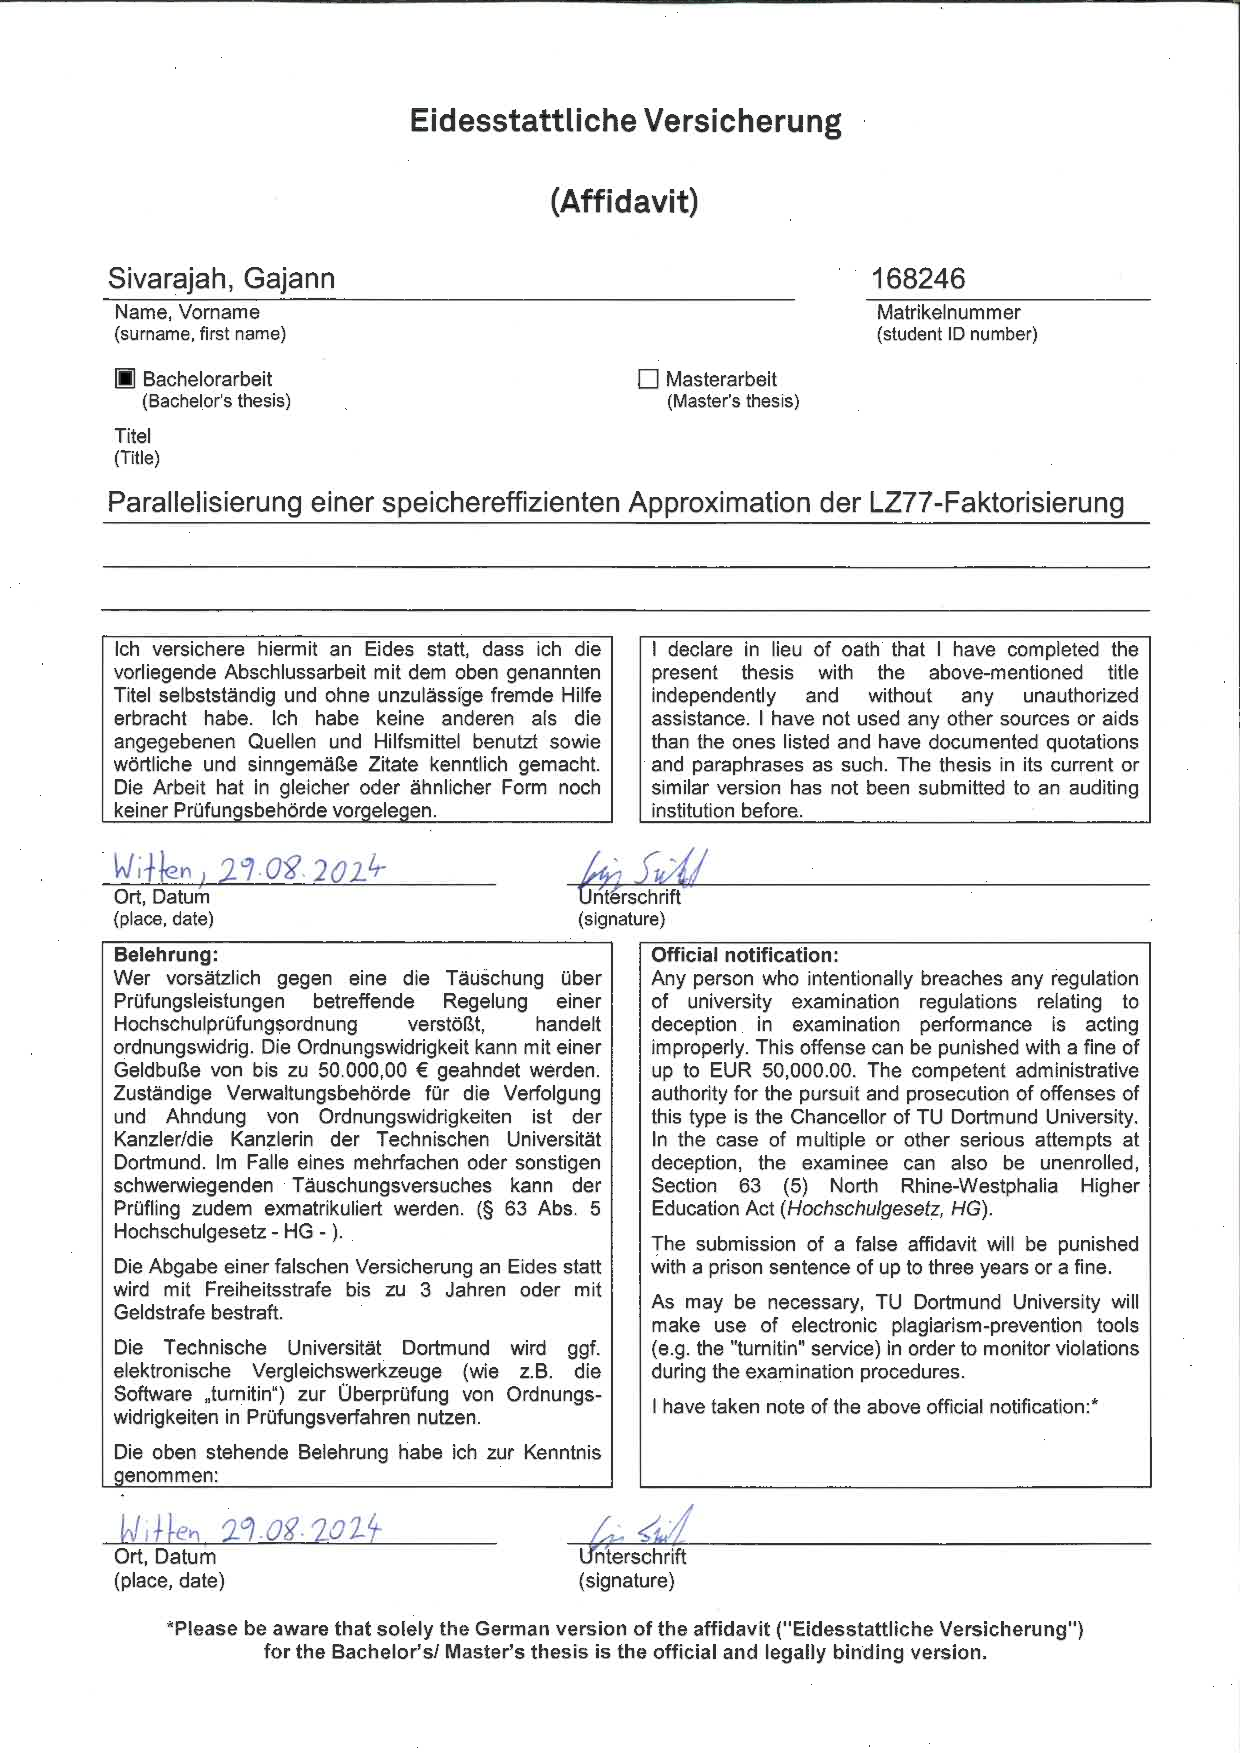
\includepdf{Chapters/Affidavit.pdf}
\cleardoublepage
\end{document}

